\section{Gestione della concorrenza}

Una base di dati deve essere gestita da più programmi contemporaneamente, e si verifica quindi il problema della concorrenza. Per misurare il carico di lavoro si utilizza il \textbf{TPS} (\textit{Transaction Per Second}), un'unità di misura che quantifica le transazioni elaborate al secondo; per gestire il sistema con prestazioni accettabili, un valore tipico di TPS è compreso tra 100 e 1000.

La concorrenza può tuttavia produrre delle \textbf{anomalie}, note come problemi di concorrenza. Per gestire tali anomalie si introducono dei meccanismi di controllo delle esecuzioni concorrenti. Il componente del DBMS preposto a questo compito è il \textbf{gestore della concorrenza}, detto anche \textbf{scheduler}, il quale riceve le richieste di accesso ai dati e decide se autorizzarle o meno; quando non le autorizza immediatamente, decide di ritardarle.
\subsection{Anomalie da esecuzione concorrente}

Le principali anomalie che possono verificarsi durante l'esecuzione concorrente di transazioni sono le seguenti:

\begin{enumerate}
	\item \textbf{Perdita di aggiornamento} (\textit{lost update}): gli effetti di una transazione vengono sovrascritti e quindi persi da un'altra transazione eseguita concorrentemente.
	\item \textbf{Lettura inconsistente} (\textit{unrepeatable read}): accessi successivi alla stessa risorsa da parte della stessa transazione restituiscono risultati diversi.
	\item \textbf{Lettura sporca} (\textit{dirty read}): viene letto un dato che rappresenta uno stato intermedio di un'altra transazione, non ancora confermato.
	\item \textbf{Aggiornamento fantasma} (\textit{phantom update}): viene osservato uno stato intermedio che viola i vincoli di integrità.
	\item \textbf{Inserimento fantasma} (\textit{phantom insert}): valutazioni diverse di operazioni di aggregazione producono risultati diversi a causa di inserimenti concorrenti.
\end{enumerate}

L'obiettivo sarebbe evitarle tutte; tuttavia, vedremo che sarà necessario adottare un compromesso tra il grado di isolamento dalle anomalie e le prestazioni della base di dati.

Utilizzeremo la seguente notazione per gli esempi:
\begin{itemize}
	\item $t_i$ per indicare una transazione.
	\item $r_i(x)$ per indicare un'operazione di lettura effettuata dalla transazione $t_i$ sulla risorsa $x$.
	\item $w_i(x)$ per indicare un'operazione di scrittura effettuata dalla transazione $t_i$ sulla risorsa $x$.
\end{itemize}
\subsubsection{Perdita di aggiornamento}

Gli effetti di una transazione concorrente vengono sovrascritti e quindi persi. Consideriamo le seguenti transazioni:
\begin{align*}
	t_1 &: \text{BOT},\ r_1(x),\ x = x+1,\ w_1(x),\ \text{commit},\ \text{EOT} \\
	t_2 &: \text{BOT},\ r_2(x),\ x = x+1,\ w_2(x),\ \text{commit},\ \text{EOT}
\end{align*}

\begin{table}[H]
	\centering
	\begin{tabular}{|c|c|c|c|c|}
		\hline
		\textbf{Op. $t_1$} & \textbf{Seg. mem. centrale $t_1$} & \textbf{Memoria secondaria} & \textbf{Seg. mem. centrale $t_2$} & \textbf{Op. $t_2$} \\
		\hline
		\multicolumn{2}{|c|}{Stato iniziale} & $x = 2$ & \multicolumn{2}{c|}{Stato iniziale} \\
		\hline
		BOT & & 2 & & \\
		\hline
		$r_1(x)$ & 2 $\leftarrow$ & {[2]} & & \\
		\hline
		$x = x+1$ & 3 & {[2]} & & \\
		\hline
		& 3 & {[2]} & & BOT \\
		\hline
		& 3 & {[2]} $\rightarrow$ & 2 & $r_2(x)$ \\
		\hline
		& 3 & {[2]} & 3 & $x = x+1$ \\
		\hline
		& 3 & {[3]} $\leftarrow$ & 3 & $w_2(x)$ \\
		\hline
		$w_1(x)$ & 3 $\rightarrow$ & {[3]} & & EOT \\
		\hline
		commit & & {[3]} & & \\
		\hline
		EOT & & \cellcolor{green!30}{[3]} & & \\
		\hline
	\end{tabular}
	\caption{Esempio di perdita di aggiornamento: $t_2$ sovrascrive il valore scritto da $t_1$.}
\end{table}
Un'esecuzione seriale delle due transazioni avrebbe prodotto il risultato corretto $x = 4$; questa esecuzione concorrente ha invece prodotto $x = 3$, a causa della sovrascrittura dell'aggiornamento di $t_2$ da parte di $t_1$. Per evitare questo tipo di anomalia è necessario ricorrere a opportune tecniche di controllo della concorrenza.
\subsubsection{Lettura inconsistente}

Accessi successivi allo stesso dato all'interno della stessa transazione producono valori diversi. Consideriamo le seguenti transazioni:
\begin{align*}
	t_1 &: \text{BOT},\ r_1(x),\ r_1'(x),\ \text{commit},\ \text{EOT} \\
	t_2 &: \text{BOT},\ r_2(x),\ x = x+1,\ w_2(x),\ \text{commit},\ \text{EOT}
\end{align*}

Si noti che in $t_1$ le operazioni $r_1(x)$ e $r_1'(x)$ rappresentano due letture successive dello stesso dato $x$ all'interno della stessa transazione.

\begin{table}[H]
	\centering
	\begin{tabular}{|c|c|c|c|c|}
		\hline
		\textbf{Op. $t_1$} & \textbf{Seg. mem. centrale $t_1$} & \textbf{Memoria secondaria} & \textbf{Seg. mem. centrale $t_2$} & \textbf{Op. $t_2$} \\
		\hline
		\multicolumn{2}{|c|}{Stato iniziale} & $x = 2$ & \multicolumn{2}{c|}{Stato iniziale} \\
		\hline
		BOT & & 2 & & \\
		\hline
		$r_1(x)$ & 2 $\leftarrow$ & 2 & & \\
		\hline
		& 2 & 2 & & BOT \\
		\hline
		& 2 & 2 $\rightarrow$ & 2 & $r_2(x)$ \\
		\hline
		& 2 & 2 & 3 & $x = x+1$ \\
		\hline
		& 2 & 3 $\leftarrow$ & 3 & $w_2(x)$ \\
		\hline
		& 2 & 3 & 3 & commit \\
		\hline
		& 2 & 3 & 3 & EOT \\
		\hline
		\rowcolor{red!15}
		$r_1'(x)$ & 3 $\leftarrow$ & 3 & & \\
		\hline
		commit & & 3 & & \\
		\hline
		EOT & & 3 & & \\
		\hline
	\end{tabular}
	\caption{Esempio di lettura inconsistente: $t_1$ legge $x = 2$ la prima volta e $x = 3$ la seconda, pur non avendo mai modificato $x$.}
\end{table}

Si può notare che il valore letto da $t_1$ per $x$ è cambiato tra la prima e la seconda lettura, nonostante $t_1$ non abbia mai modificato $x$.
\subsubsection{Lettura sporca}

Viene letto un dato che rappresenta uno stato intermedio nell'evoluzione di una transazione. Consideriamo le seguenti transazioni:
\begin{align*}
	t_1 &: \text{BOT},\ r_1(x),\ \text{commit},\ \text{EOT} \\
	t_2 &: \text{BOT},\ r_2(x),\ x = x+1,\ w_2(x),\ \text{abort},\ \text{EOT}
\end{align*}

Poiché $t_2$ esegue un \textbf{abort}, la transazione viene annullata e i suoi effetti sulla base di dati vengono ripristinati (\textit{rollback}): è come se $t_2$ non fosse mai stata eseguita.

\begin{table}[H]
	\centering
	\begin{tabular}{|c|c|c|c|c|}
		\hline
		\textbf{Op. $t_1$} & \textbf{Mem. centr. $t_1$} & \textbf{Memoria secondaria} & \textbf{Mem. centr. $t_2$} & \textbf{Op. $t_2$} \\
		\hline
		\multicolumn{2}{|c|}{Stato iniziale} & $x = 2$ & \multicolumn{2}{c|}{Stato iniziale} \\
		\hline
		BOT & & 2 & & \\
		\hline
		& & 2 & & BOT \\
		\hline
		& & 2 $\rightarrow$ & 2 & $r_2(x)$ \\
		\hline
		& & 2 & 3 & $x = x+1$ \\
		\hline
		& & 3 $\leftarrow$ & 3 & $w_2(x)$ \\
		\hline
		\rowcolor{red!15}
		$r_1(x)$ & 3 $\leftarrow$ & 3 & & \\
		\hline
		\rowcolor{red!15}
		commit & \textcolor{red}{3} & \textcolor{red}{2} & & abort \\
		\hline
		EOT & & 2 & & EOT \\
		\hline
	\end{tabular}
	\caption{Esempio di lettura sporca: $t_1$ legge il valore $x = 3$ scritto da $t_2$, che però esegue abort e ripristina $x = 2$.}
\end{table}

Il valore 3 letto da $t_1$ non è conforme al contenuto reale della memoria secondaria: poiché $t_2$ ha eseguito l'abort, i suoi effetti sono stati annullati e il valore corretto di $x$ rimane 2. $t_1$ ha quindi letto uno stato intermedio che non avrebbe dovuto essere visibile.
\subsubsection{Aggiornamento fantasma}

Osservazione di uno stato intermedio che non soddisfa i vincoli di integrità. Supponiamo di avere tre risorse $x$, $y$, $z$ con il vincolo che la loro somma debba essere maggiore o uguale a 100:
\[
x + y + z \geq 100
\]

Consideriamo le seguenti transazioni:
\begin{align*}
	t_1 &: \text{BOT},\ r_1(y),\ r_1(x),\ r_1(z),\ S = x+y+z,\ \text{EOT} \\
	t_2 &: \text{BOT},\ r_2(y),\ y = y+10,\ r_2(z),\ z = z-10,\ w_2(y),\ w_2(z),\ \text{commit},\ \text{EOT}
\end{align*}

Si noti che $t_2$ non viola il vincolo: sposta semplicemente 10 unità da $z$ a $y$, lasciando invariata la somma. Tuttavia, a causa dell'interleaving, $t_1$ può osservare uno stato intermedio in cui il vincolo risulta violato.

\begin{table}[H]
	\centering
	\begin{tabular}{|c|c|c|c|c|}
		\hline
		\textbf{Op. $t_1$} & \textbf{Mem. centr. $t_1$} & \textbf{Memoria secondaria} & \textbf{Mem. centr. $t_2$} & \textbf{Op. $t_2$} \\
		\hline
		\multicolumn{2}{|c|}{Stato iniziale} & $(x,y,z) = 20, 20, 60$ & \multicolumn{2}{c|}{Stato iniziale} \\
		\hline
		BOT & & 20, 20, 60 & & \\
		\hline
		$r_1(y)$ & $-,20,-$ $\leftarrow$ & 20, 20, 60 & & \\
		\hline
		& $-,20,-$ & 20, 20, 60 & & BOT \\
		\hline
		& $-,20,-$ & 20, 20, 60 $\rightarrow$ & $-,20,-$ & $r_2(y)$ \\
		\hline
		& $-,20,-$ & 20, 20, 60 & $-,30,-$ & $y = y+10$ \\
		\hline
		& $-,20,-$ & 20, 20, 60 $\rightarrow$ & $-,30,60$ & $r_2(z)$ \\
		\hline
		& $-,20,-$ & 20, 20, 60 & $-,30,50$ & $z = z-10$ \\
		\hline
		& $-,20,-$ & 20, 30, 60 $\leftarrow$ & $-,30,50$ & $w_2(y)$ \\
		\hline
		& $-,20,-$ & \cellcolor{yellow!40}20, 30, 50 $\leftarrow$ & $-,30,50$ & $w_2(z)$ \\
		\hline
		& $-,20,-$ & \cellcolor{yellow!40}20, 30, 50 & & commit \textcolor{green!50!black}{(vincolo OK)} \\
		\hline
		\rowcolor{red!15}
		$r_1(x)$ & 20, 20, 50 & \cellcolor{yellow!40}20, 30, 50 & & \\
		\hline
		\rowcolor{red!15}
		$r_1(z)$ & 20, 20, 50 &  & & \textcolor{red}{vincolo violato per $t_1$!} \\
		\hline
	\end{tabular}
	\caption{Aggiornamento fantasma: $t_2$ non viola il vincolo, ma $t_1$ osserva uno stato intermedio in cui $x + y + z = 20 + 20 + 50 = 90 < 100$.}
\end{table}
\subsubsection{Inserimento fantasma}

Valutazioni diverse di operatori di aggregazione ($\text{SUM}$, $\text{COUNT}$, $\text{AVG}$, $\text{MAX}$, $\text{MIN}$) all'interno della stessa transazione producono risultati diversi. È un'anomalia simile alla lettura inconsistente, ma coinvolge operatori di aggregazione anziché singoli valori.

La differenza sostanziale rispetto alle anomalie precedenti risiede nella natura della risorsa coinvolta: non si tratta di un singolo dato, ma dell'intera tabella. L'anomalia si manifesta quando, tra due valutazioni successive dello stesso operatore di aggregazione, un'altra transazione inserisce nuove tuple, alterando il risultato.
\subsection{Schedule}

Uno \textbf{schedule} è una sequenza di operazioni di lettura e scrittura eseguite su risorse della base di dati da transazioni concorrenti. Date le seguenti transazioni:
\begin{align*}
	t_1 &: \text{BOT},\ r_1(x),\ w_1(x),\ \text{commit},\ \text{EOT} \\
	t_2 &: \text{BOT},\ r_2(x),\ w_2(x),\ \text{commit},\ \text{EOT}
\end{align*}

Un possibile schedule è ad esempio:
\[
S: r_1(x),\ r_2(x),\ w_2(x),\ w_1(x)
\]

Date due o più transazioni, esistono più schedule possibili. L'obiettivo è accettare solo gli schedule che evitano le anomalie, ovvero gli schedule equivalenti a uno schedule seriale.

Uno \textbf{schedule seriale} è uno schedule in cui le operazioni di ogni transazione compaiono in sequenza, senza essere inframmezzate da operazioni di altre transazioni. Ad esempio:
\begin{align*}
	S_1 &: r_1(x),\ r_2(x),\ w_2(x),\ w_1(x) \quad \text{(non seriale)} \\
	S_2 &: r_1(x),\ w_1(x),\ r_2(x),\ w_2(x) \quad \text{(seriale)} \\
	S_3 &: r_2(x),\ w_2(x),\ r_1(x),\ w_1(x) \quad \text{(seriale)}
\end{align*}

L'obiettivo del gestore della concorrenza è individuare gli schedule \textbf{serializzabili}, ovvero equivalenti a uno schedule seriale. Per equivalenza si intende che lo schedule produce lo stesso effetto sulla base di dati che si otterrebbe eseguendo le transazioni una di seguito all'altra. È quindi necessario definire formalmente quando uno schedule è equivalente a uno schedule seriale.
\subsubsection{Ipotesi di commit-proiezione}

Per semplificare l'analisi, supponiamo che l'esito di tutte le transazioni sia noto a priori. In base a questa ipotesi, escludiamo dagli schedule le operazioni delle transazioni che terminano con un abort, considerando quindi solo le transazioni che giungono a buon fine con un commit.

Introdurremo due nozioni di equivalenza tra schedule:
\begin{enumerate}
	\item \textbf{View equivalenza}
	\item \textbf{Conflict equivalenza}
\end{enumerate}
\subsubsection{View-Equivalenza}

La view equivalenza si basa su due relazioni fondamentali: \textit{legge-da} e \textit{scritture finali}.

\paragraph{Relazione legge-da.}
Dato uno schedule $S$, si dice che un'operazione di lettura $r_i(x)$ \textbf{legge-da} un'operazione di scrittura $w_j(x)$ se:
\begin{enumerate}
	\item $w_j(x)$ precede $r_i(x)$ in $S$;
	\item $j \neq i$;
	\item non esiste alcuna operazione $w_k(x)$ tra $w_j(x)$ e $r_i(x)$, ovvero $w_j(x)$ è la scrittura di $x$ immediatamente precedente a $r_i(x)$.
\end{enumerate}

Consideriamo i seguenti esempi:
\begin{align*}
	S_1 &: r_1(x),\ r_2(x),\ w_2(x),\ w_1(x) \quad \Rightarrow \quad \text{LEGGE\_DA}(S_1) = \emptyset \\
	& \text{\small($r_1(x)$ non è preceduta da alcuna scrittura; $r_2(x)$ è preceduta solo da $r_1(x)$, non da una scrittura)} \\[4pt]
	S_2 &: r_1(x),\ w_1(x),\ r_2(x),\ w_2(x) \quad \Rightarrow \quad \text{LEGGE\_DA}(S_2) = \{(r_2(x),\ w_1(x))\} \\
	& \text{\small($r_2(x)$ è preceduta da $w_1(x)$, che è la scrittura di $x$ immediatamente precedente)} \\[4pt]
	S_3 &: r_1(x),\ w_1(x),\ w_2(x),\ r_1(x) \quad \Rightarrow \quad \text{LEGGE\_DA}(S_3) = \emptyset \\
	& \text{\small(la seconda $r_1(x)$ è preceduta da $w_2(x)$, ma $i = 1 = k$, quindi la condizione $j \neq i$ non è soddisfatta)}
\end{align*}

\paragraph{Relazione scritture finali.}
Dato uno schedule $S$, un'operazione di scrittura $w_i(x)$ è una \textbf{scrittura finale} se è l'ultima operazione di scrittura su $x$ in $S$. Per ogni risorsa si individua quindi l'ultima transazione che ha effettuato una scrittura su di essa:
\[
S_1 : r_1(x),\ r_2(x),\ w_2(x),\ w_3(y),\ w_1(x) \quad \Rightarrow \quad \text{SCRITTURE\_FINALI}(S_1) = \{w_1(x),\ w_3(y)\}
\]

\paragraph{Definizione di view equivalenza.}
Due schedule $S_1$ e $S_2$ sono \textbf{view-equivalenti} ($S_1 \approx_V S_2$) se e solo se possiedono lo stesso insieme legge-da e lo stesso insieme di scritture finali.

Uno schedule $S$ è \textbf{view-serializzabile} se è view-equivalente a uno schedule seriale.
\paragraph{Esempio: perdita di aggiornamento.}

Consideriamo le transazioni:
\begin{align*}
	t_1 &: r_1(x),\ w_1(x) \\
	t_2 &: r_2(x),\ w_2(x)
\end{align*}

Uno schedule che rappresenta la perdita di aggiornamento è:
\[
S_{pa} : r_1(x),\ r_2(x),\ w_2(x),\ w_1(x)
\]

Calcoliamo le relazioni:
\begin{itemize}
	\item $\text{LEGGE\_DA}(S_{pa}) = \emptyset$: né $r_1(x)$ né $r_2(x)$ sono precedute da alcuna scrittura sullo stesso dato, quindi nessuna lettura legge-da una scrittura.
	\item $\text{SCRITTURE\_FINALI}(S_{pa}) = \{w_1(x)\}$: l'ultima operazione di scrittura su $x$ è $w_1(x)$, che compare per ultima tra le scritture.
\end{itemize}

Per determinare se $S_{pa}$ è view-serializzabile, dobbiamo verificare se esiste uno schedule seriale view-equivalente. Gli unici schedule seriali possibili sono:

\[
S_{12} : r_1(x),\ w_1(x),\ r_2(x),\ w_2(x)
\]
\begin{itemize}
	\item $\text{LEGGE\_DA}(S_{12}) = \{(r_2(x),\ w_1(x))\}$: $r_2(x)$ è preceduta immediatamente da $w_1(x)$.
	\item $\text{SCRITTURE\_FINALI}(S_{12}) = \{w_2(x)\}$: l'ultima scrittura su $x$ è $w_2(x)$.
\end{itemize}
$S_{12}$ non è view-equivalente a $S_{pa}$: differiscono sia nell'insieme legge-da che nelle scritture finali.

\[
S_{21} : r_2(x),\ w_2(x),\ r_1(x),\ w_1(x)
\]
\begin{itemize}
	\item $\text{LEGGE\_DA}(S_{21}) = \{(r_1(x),\ w_2(x))\}$: $r_1(x)$ è preceduta immediatamente da $w_2(x)$.
	\item $\text{SCRITTURE\_FINALI}(S_{21}) = \{w_1(x)\}$: l'ultima scrittura su $x$ è $w_1(x)$.
\end{itemize}
$S_{21}$ non è view-equivalente a $S_{pa}$: pur avendo le stesse scritture finali, l'insieme legge-da è diverso.

Poiché nessuno dei due schedule seriali è view-equivalente a $S_{pa}$, possiamo concludere che $\mathbf{S_{pa}}$ \textbf{non è view-serializzabile}.
\paragraph{Esempio: lettura inconsistente.}

Consideriamo le transazioni:
\begin{align*}
	t_1 &: r_1(x),\ r_1'(x) \\
	t_2 &: r_2(x),\ w_2(x)
\end{align*}

Lo schedule che rappresenta la lettura inconsistente è:
\[
S_{li} : r_1(x),\ r_2(x),\ w_2(x),\ r_1'(x)
\]

\begin{itemize}
	\item $\text{LEGGE\_DA}(S_{li}) = \{(r_1'(x),\ w_2(x))\}$: $r_1'(x)$ è preceduta immediatamente da $w_2(x)$, mentre $r_1(x)$ non è preceduta da alcuna scrittura.
	\item $\text{SCRITTURE\_FINALI}(S_{li}) = \{w_2(x)\}$: l'unica scrittura su $x$ è $w_2(x)$, che è quindi anche l'ultima.
\end{itemize}

Gli schedule seriali possibili sono:

\[
S_{12} : r_1(x),\ r_1'(x),\ r_2(x),\ w_2(x)
\]
\begin{itemize}
	\item $\text{LEGGE\_DA}(S_{12}) = \emptyset$: nessuna lettura è preceduta da una scrittura.
	\item $\text{SCRITTURE\_FINALI}(S_{12}) = \{w_2(x)\}$.
\end{itemize}
$S_{12}$ non è view-equivalente a $S_{li}$: l'insieme legge-da è diverso.

\[
S_{21} : r_2(x),\ w_2(x),\ r_1(x),\ r_1'(x)
\]
\begin{itemize}
	\item $\text{LEGGE\_DA}(S_{21}) = \{(r_1(x),\ w_2(x)),\ (r_1'(x),\ w_2(x))\}$: sia $r_1(x)$ che $r_1'(x)$ sono precedute immediatamente da $w_2(x)$.
	\item $\text{SCRITTURE\_FINALI}(S_{21}) = \{w_2(x)\}$.
\end{itemize}
$S_{21}$ non è view-equivalente a $S_{li}$: pur avendo le stesse scritture finali, l'insieme legge-da differisce — $S_{li}$ contiene solo $(r_1'(x),\ w_2(x))$, mentre $S_{21}$ contiene anche $(r_1(x),\ w_2(x))$.

Poiché $S_{li}$ non è view-equivalente ad alcuno schedule seriale, concludiamo che $\mathbf{S_{li}}$ \textbf{non è view-serializzabile}.
\paragraph{Esempio: verifica di view-serializzabilità.}

Consideriamo lo schedule:
\[
S_1 : r_1(x),\ w_1(x),\ r_2(z),\ r_1(y),\ w_1(y),\ r_2(x),\ w_2(x),\ w_2(z)
\]

Le transazioni coinvolte sono:
\begin{align*}
	t_1 &: r_1(x),\ w_1(x),\ r_1(y),\ w_1(y) \\
	t_2 &: r_2(z),\ r_2(x),\ w_2(x),\ w_2(z)
\end{align*}

Calcoliamo le relazioni per $S_1$:
\begin{itemize}
	\item $\text{LEGGE\_DA}(S_1) = \{(r_2(x),\ w_1(x))\}$: $r_2(x)$ è preceduta immediatamente da $w_1(x)$; $r_1(y)$, $r_2(z)$ e $r_1(x)$ non sono precedute da alcuna scrittura.
	\item $\text{SCRITTURE\_FINALI}(S_1) = \{w_2(x),\ w_1(y),\ w_2(z)\}$: $w_2(x)$ è l'ultima scrittura su $x$, $w_1(y)$ l'unica su $y$, $w_2(z)$ l'unica su $z$.
\end{itemize}

Gli schedule seriali possibili sono $S_{12}$ (prima $t_1$, poi $t_2$) e $S_{21}$ (prima $t_2$, poi $t_1$). Possiamo escludere immediatamente $S_{21}$: in $S_1$ la relazione legge-da impone $t_1 < t_2$ (poiché $r_2(x)$ legge-da $w_1(x)$), e le scritture finali impongono anch'esse $t_1 < t_2$ su $w_2(x)$; in $S_{21}$ l'ordine sarebbe invertito, quindi non può essere view-equivalente.

Verifichiamo $S_{12}$:
\[
S_{12} : r_1(x),\ w_1(x),\ r_1(y),\ w_1(y),\ r_2(z),\ r_2(x),\ w_2(x),\ w_2(z)
\]
\begin{itemize}
	\item $\text{LEGGE\_DA}(S_{12}) = \{(r_2(x),\ w_1(x))\}$
	\item $\text{SCRITTURE\_FINALI}(S_{12}) = \{w_2(x),\ w_1(y),\ w_2(z)\}$
\end{itemize}

Poiché $\text{LEGGE\_DA}(S_1) = \text{LEGGE\_DA}(S_{12})$ e $\text{SCRITTURE\_FINALI}(S_1) = \text{SCRITTURE\_FINALI}(S_{12})$, concludiamo che $S_1 \approx_V S_{12}$, quindi $\mathbf{S_1}$ \textbf{è view-serializzabile}.
\paragraph{Esempio: schedule non view-serializzabile.}

Consideriamo lo schedule:
\[
S_2 : r_1(x),\ w_1(x),\ w_3(x),\ r_2(y),\ r_3(y),\ w_3(y),\ w_1(y),\ r_2(x)
\]

Le transazioni coinvolte sono:
\begin{align*}
	t_1 &: r_1(x),\ w_1(x),\ w_1(y) \\
	t_2 &: r_2(y),\ r_2(x) \\
	t_3 &: w_3(x),\ r_3(y),\ w_3(y)
\end{align*}

Calcoliamo le relazioni per $S_2$:
\begin{itemize}
	\item $\text{LEGGE\_DA}(S_2) = \{(r_2(x),\ w_3(x))\}$: $r_2(x)$ è preceduta immediatamente da $w_3(x)$.
	\item $\text{SCRITTURE\_FINALI}(S_2) = \{w_3(x),\ w_1(y)\}$: $w_3(x)$ è l'ultima scrittura su $x$, $w_1(y)$ è l'ultima scrittura su $y$.
\end{itemize}

In linea di principio occorrerebbe esaminare tutte le $6$ permutazioni seriali possibili. Tuttavia, l'insieme delle scritture finali ci permette di escluderle tutte a priori imponendo due vincoli sull'ordine delle transazioni:
\begin{itemize}
	\item $w_3(x) \in \text{SCRITTURE\_FINALI}$ impone $t_1 < t_3$, affinché $w_1(x)$ non sovrascriva $w_3(x)$;
	\item $w_1(y) \in \text{SCRITTURE\_FINALI}$ impone $t_3 < t_1$, affinché $w_3(y)$ non sovrascriva $w_1(y)$.
\end{itemize}

I due vincoli sono contraddittori: non può esistere uno schedule seriale che soddisfi contemporaneamente $t_1 < t_3$ e $t_3 < t_1$. Pertanto, nessuna delle sei permutazioni può essere view-equivalente a $S_2$, e concludiamo che $\mathbf{S_2}$ \textbf{non è view-serializzabile}.
\paragraph{Esempio: schedule con 5 transazioni.}

Consideriamo lo schedule:
\[
S_3 : r_1(x),\ r_2(x),\ w_2(x),\ r_3(x),\ r_4(z),\ w_1(x),\ w_3(y),\ w_3(x),\ w_1(y),\ w_5(x),\ w_1(z),\ w_5(y),\ r_5(z)
\]

Le transazioni coinvolte sono:
\begin{align*}
	t_1 &: r_1(x),\ w_1(x),\ w_1(y),\ w_1(z) \\
	t_2 &: r_2(x),\ w_2(x) \\
	t_3 &: r_3(x),\ w_3(y),\ w_3(x) \\
	t_4 &: r_4(z) \\
	t_5 &: w_5(x),\ w_5(y),\ r_5(z)
\end{align*}

Calcoliamo le relazioni per $S_3$:
\begin{itemize}
	\item $\text{LEGGE\_DA}(S_3) = \{(r_3(x),\ w_2(x)),\ (r_5(z),\ w_1(z))\}$
	\item $\text{SCRITTURE\_FINALI}(S_3) = \{w_5(x),\ w_5(y),\ w_1(z)\}$
\end{itemize}

Ricaviamo ora i vincoli sull'ordine delle transazioni in qualsiasi schedule seriale view-equivalente a $S_3$.

\textbf{Dalle scritture finali:}
\begin{itemize}
	\item $w_5(x) \in \text{SCRITTURE\_FINALI}$ impone $t_2 < t_5$,\ $t_1 < t_5$,\ $t_3 < t_5$;
	\item $w_5(y) \in \text{SCRITTURE\_FINALI}$ impone $t_3 < t_5$,\ $t_1 < t_5$;
	\item $w_1(z) \in \text{SCRITTURE\_FINALI}$ non aggiunge vincoli ulteriori.
\end{itemize}

\textbf{Dall'insieme legge-da:}
\begin{itemize}
	\item $(r_3(x),\ w_2(x)) \in \text{LEGGE\_DA}$ impone $t_2 < t_3$, affinché $r_3(x)$ legga da $w_2(x)$;
	\item $(r_5(z),\ w_1(z)) \in \text{LEGGE\_DA}$ impone $t_1 < t_5$.
\end{itemize}

\textbf{Dalla non appartenenza a legge-da:}
Poiché $r_2(x)$ precede fisicamente $w_1(x)$ in $S_3$ e $(r_2(x),\ w_1(x)) \notin \text{LEGGE\_DA}(S_3)$, in qualsiasi schedule seriale equivalente $t_2$ deve precedere $t_1$, affinché $r_2(x)$ non legga da $w_1(x)$:
\[
t_2 < t_1
\]

\textbf{Contraddizione:} i vincoli ricavati impongono simultaneamente $t_2 < t_3$, $t_2 < t_1$ e $t_1 < t_5$, ma dall'insieme legge-da avevamo già ricavato $t_2 < t_3$ con $t_1 < t_2$ implicato dalla struttura dello schedule — il che genera un ciclo $t_2 < t_1 < t_2$. Non esiste quindi alcuno schedule seriale che soddisfi tutti i vincoli contemporaneamente, e concludiamo che $\mathbf{S_3}$ \textbf{non è view-serializzabile}.
\subsection{Conflict equivalenza}

\paragraph{Conflitto.}
Dato uno schedule $S$, si dice che una coppia di operazioni $(a_i, a_j)$ rappresenta un \textbf{conflitto} se:
\begin{itemize}
	\item $i \neq j$, ovvero le operazioni appartengono a transazioni diverse;
	\item entrambe operano sulla stessa risorsa;
	\item almeno una delle due è un'operazione di scrittura;
	\item $a_i$ compare prima di $a_j$ in $S$.
\end{itemize}

\paragraph{Conflict equivalenza.}
Due schedule $S_1$ e $S_2$ sono \textbf{conflict-equivalenti} ($S_1 \approx_C S_2$) se e solo se possiedono lo stesso insieme di conflitti.
\paragraph{Conflict-serializzabilità.}

Uno schedule $S$ è \textbf{conflict-serializzabile} (CSR) se esiste uno schedule seriale $S_r$ tale che $S \approx_C S_r$. Il vantaggio rispetto alla view-serializzabilità è che l'algoritmo per il test della conflict-serializzabilità ha complessità \textbf{lineare}.

\paragraph{Algoritmo CSR.}

Dato uno schedule $S$, l'algoritmo procede come segue:
\begin{enumerate}
	\item Costruire l'insieme dei conflitti di $S$.
	\item Costruire il \textbf{grafo dei conflitti} $G(N, A)$, dove:
	\begin{itemize}
		\item $N$ è l'insieme dei nodi, uno per ciascuna transazione di $S$;
		\item $A$ contiene un arco $(t_i, t_j)$ se esiste un conflitto $(a_i, a_j) \in S$.
	\end{itemize}
	\item Se il grafo dei conflitti è \textbf{aciclico}, allora $S$ è conflict-serializzabile; altrimenti non lo è.
\end{enumerate}

\paragraph{Dimostrazione di correttezza.}

\textbf{($\Rightarrow$) Se $S$ è CSR allora il suo grafo è aciclico.}
Sia $S_r$ lo schedule seriale conflict-equivalente a $S$, con le transazioni ordinate $t_1, t_2, \ldots, t_n$. Poiché $S \approx_C S_r$, i due schedule hanno esattamente gli stessi conflitti nello stesso ordine. Nel grafo dei conflitti di $S_r$ possono quindi comparire solo archi $(t_i, t_j)$ con $i < j$: un ciclo richiederebbe un arco $(t_j, t_i)$ con $j > i$, che implicherebbe l'esistenza di un conflitto in ordine inverso — impossibile in uno schedule seriale. Poiché $S$ e $S_r$ hanno lo stesso grafo, anche il grafo di $S$ è aciclico.

\textbf{($\Leftarrow$) Se il grafo di $S$ è aciclico allora $S$ è CSR.}
Se il grafo è aciclico, esiste un \textbf{ordinamento topologico}, ovvero una numerazione dei nodi tale che il grafo contenga solo archi $(t_i, t_j)$ con $i < j$. Utilizzando questo ordinamento topologico possiamo definire un ordine delle transazioni che produce lo stesso grafo dei conflitti di $S$: otteniamo così uno schedule seriale $S_r$ conflict-equivalente a $S$, quindi $S$ è CSR.

\paragraph{Esempio CSR: perdita di aggiornamento.}

Consideriamo lo schedule $S_{pa}$ già visto in precedenza:
\[
S_{pa} : r_1(x),\ r_2(x),\ w_2(x),\ w_1(x)
\]

Costruiamo l'insieme dei conflitti:
\[
\text{CONFLITTI}(S_{pa}) = \{(r_1(x),\ w_2(x)),\ (r_2(x),\ w_1(x)),\ (w_2(x),\ w_1(x))\}
\]
\begin{itemize}
	\item $(r_1(x),\ w_2(x))$: $r_1$ e $w_2$ operano sulla stessa risorsa $x$, appartengono a transazioni diverse, e $w_2$ è una scrittura;
	\item $(r_2(x),\ w_1(x))$: analogo, con $w_1$ scrittura;
	\item $(w_2(x),\ w_1(x))$: entrambe scritture sulla stessa risorsa $x$, transazioni diverse.
\end{itemize}
\begin{figure}[H]
	\centering
	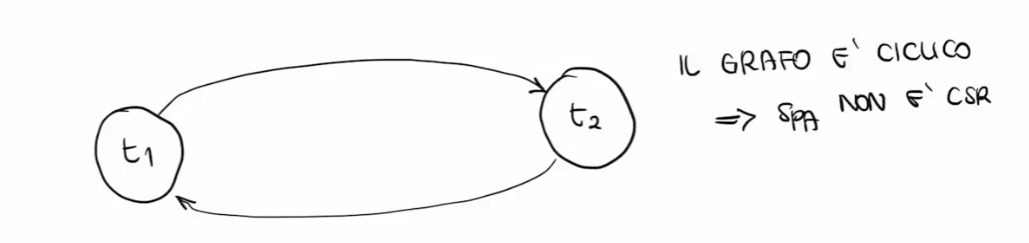
\includegraphics[width=0.7\linewidth]{image240}
	\label{fig:image240}
\end{figure}
Dal primo conflitto otteniamo un arco $t_1 \to t_2$; dal secondo e dal terzo un arco $t_2 \to t_1$. Il grafo dei conflitti contiene quindi un ciclo $t_1 \to t_2 \to t_1$, pertanto $\mathbf{S_{pa}}$ \textbf{non è CSR}.
\paragraph{Esempio CSR: lettura inconsistente.}

Consideriamo le transazioni:
\begin{align*}
	t_1 &: r_1(x),\ r_1'(x) \\
	t_2 &: r_2(x),\ w_2(x)
\end{align*}

Lo schedule è:
\[
S_{li} : r_1(x),\ r_2(x),\ w_2(x),\ r_1'(x)
\]

Costruiamo l'insieme dei conflitti:
\[
\text{CONFLITTI}(S_{li}) = \{(r_1(x),\ w_2(x)),\ (w_2(x),\ r_1'(x))\}
\]
\begin{itemize}
	\item $(r_1(x),\ w_2(x))$: $r_1$ precede $w_2$, stessa risorsa $x$, transazioni diverse, $w_2$ è scrittura $\Rightarrow$ arco $t_1 \to t_2$;
	\item $(w_2(x),\ r_1'(x))$: $w_2$ precede $r_1'$, stessa risorsa $x$, transazioni diverse, $w_2$ è scrittura $\Rightarrow$ arco $t_2 \to t_1$.
\end{itemize}
\begin{figure}[H]
	\centering
	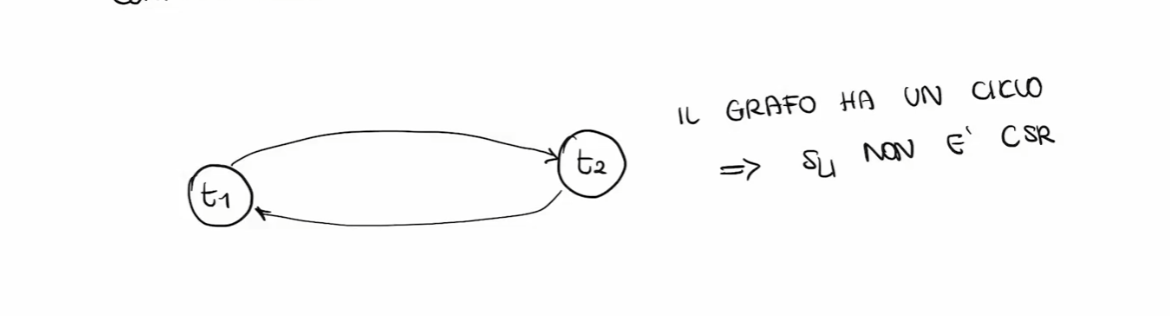
\includegraphics[width=1\linewidth]{image241}
	\label{fig:image241}
\end{figure}
Il grafo dei conflitti contiene un ciclo $t_1 \to t_2 \to t_1$, pertanto $\mathbf{S_{li}}$ \textbf{non è CSR}.
\subsection{Relazione tra CSR e VSR}

La conflict-serializzabilità è una condizione \textbf{sufficiente ma non necessaria} per la view-serializzabilità. In altri termini:

\begin{itemize}
	\item $S \in \text{CSR} \Rightarrow S \in \text{VSR}$: se uno schedule è conflict-serializzabile, allora è anche view-serializzabile.
	\item $S \notin \text{CSR} \not\Rightarrow S \notin \text{VSR}$: se uno schedule non è conflict-serializzabile, non possiamo concludere nulla sulla sua view-serializzabilità.
	\item $S \notin \text{VSR} \Rightarrow S \notin \text{CSR}$: se uno schedule non è view-serializzabile, allora non è nemmeno conflict-serializzabile.
\end{itemize}

Quindi l'insieme CSR è un sottoinsieme proprio di VSR: esistono schedule view-serializzabili che non sono conflict-serializzabili, ma non viceversa.

\paragraph{Strategia per gli esercizi.}
Data uno schedule $S$, la procedura da seguire è:
\begin{enumerate}
	\item Applicare il \textbf{test CSR}: costruire il grafo dei conflitti e verificare se è aciclico.
	\begin{itemize}
		\item Se $S$ è CSR $\Rightarrow$ $S$ è anche VSR. Non è necessario proseguire.
		\item Se $S$ non è CSR $\Rightarrow$ applicare il \textbf{test VSR} per determinare se $S$ è comunque view-serializzabile.
	\end{itemize}
\end{enumerate}
\paragraph{Esempio CSR: schedule $S_1$.}

Riprendiamo lo schedule già analizzato in precedenza:
\[
S_1 : r_1(x),\ w_1(x),\ r_2(z),\ r_1(y),\ w_1(y),\ r_2(x),\ w_2(x),\ w_2(z)
\]

Costruiamo l'insieme dei conflitti:
\[
\text{CONFLITTI}(S_1) = \{(r_1(x),\ w_2(x)),\ (w_1(x),\ r_2(x)),\ (w_1(x),\ w_2(x))\}
\]
\begin{itemize}
	\item $(r_1(x),\ w_2(x))$: $r_1$ precede $w_2$, stessa risorsa $x$, transazioni diverse, $w_2$ è scrittura $\Rightarrow$ arco $t_1 \to t_2$;
	\item $(w_1(x),\ r_2(x))$: $w_1$ precede $r_2$, stessa risorsa $x$, transazioni diverse, $w_1$ è scrittura $\Rightarrow$ arco $t_1 \to t_2$;
	\item $(w_1(x),\ w_2(x))$: entrambe scritture su $x$, transazioni diverse, $w_1$ precede $w_2$ $\Rightarrow$ arco $t_1 \to t_2$.
\end{itemize}
\begin{figure}[H]
	\centering
	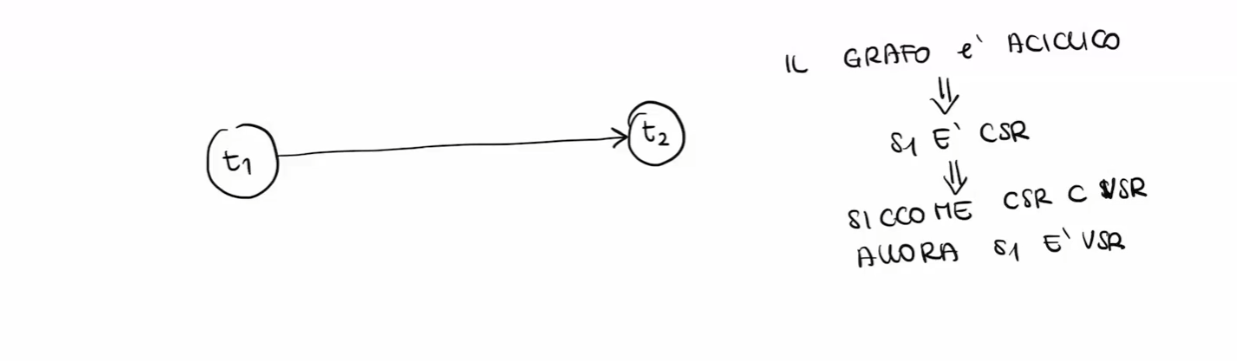
\includegraphics[width=1\linewidth]{image242}
	\label{fig:image242}
\end{figure}
Tutti e tre i conflitti generano archi nella stessa direzione $t_1 \to t_2$. Il grafo dei conflitti è quindi aciclico, pertanto $S_1$ è CSR. Poiché $\text{CSR} \subseteq \text{VSR}$, concludiamo che $\mathbf{S_1}$ \textbf{è sia CSR che VSR}.

\paragraph{Esempio CSR: schedule $S_2$.}

Riprendiamo lo schedule $S_2$ già analizzato in precedenza:
\[
S_2 : r_1(x),\ w_1(x),\ w_3(x),\ r_2(y),\ r_3(y),\ w_3(y),\ w_1(y),\ r_2(x)
\]

Costruiamo l'insieme dei conflitti:
\[
\text{CONFLITTI}(S_2) = \{
(r_1(x),\ w_3(x)),\
(w_1(x),\ w_3(x)),\
(w_1(x),\ r_2(x)),\
(w_3(x),\ r_2(x)),\
(r_2(y),\ w_3(y)),\
(r_2(y),\ w_1(y)),\
(r_3(y),\ w_1(y)),\
(w_3(y),\ w_1(y))
\}
\]

Ricaviamo gli archi del grafo dei conflitti:
\begin{itemize}
	\item $(r_1(x),\ w_3(x))$, $(w_1(x),\ w_3(x))$ $\Rightarrow$ arco $t_1 \to t_3$;
	\item $(w_1(x),\ r_2(x))$ $\Rightarrow$ arco $t_1 \to t_2$;
	\item $(w_3(x),\ r_2(x))$ $\Rightarrow$ arco $t_3 \to t_2$;
	\item $(r_2(y),\ w_3(y))$ $\Rightarrow$ arco $t_2 \to t_3$;
	\item $(r_2(y),\ w_1(y))$ $\Rightarrow$ arco $t_2 \to t_1$;
	\item $(r_3(y),\ w_1(y))$, $(w_3(y),\ w_1(y))$ $\Rightarrow$ arco $t_3 \to t_1$.
\end{itemize}

\begin{figure}[H]
	\centering
	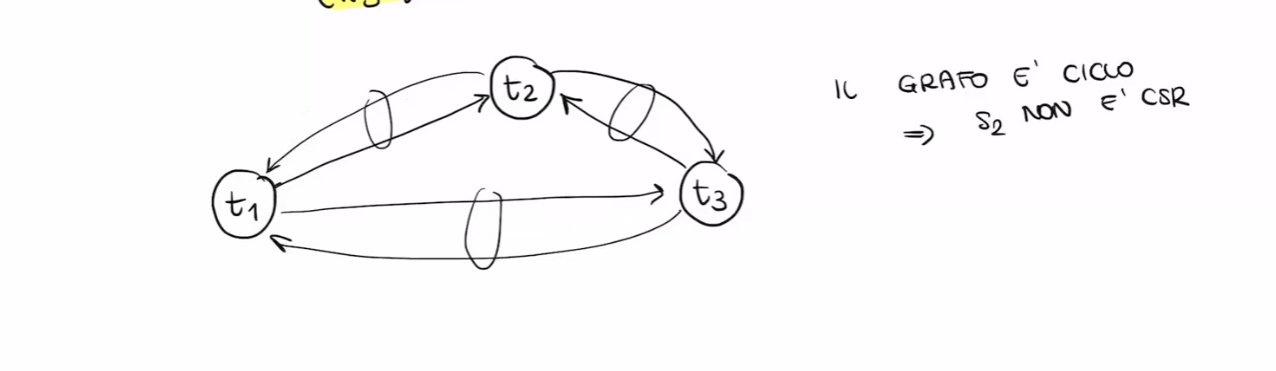
\includegraphics[width=1\linewidth]{image243}
	\label{fig:image243}
\end{figure}
Il grafo dei conflitti contiene cicli: $t_2 \to t_3 \to t_2$ e $t_1 \to t_3 \to t_1$. Il grafo è quindi ciclico, pertanto $S_2$ non è CSR. Poiché $\text{CSR} \subseteq \text{VSR}$ e avevamo già dimostrato che $S_2$ non è VSR, possiamo concludere che $\mathbf{S_2}$ \textbf{non è né CSR né VSR}.
\paragraph{Esempio CSR: schedule $S_3$.}

Riprendiamo lo schedule $S_3$ già analizzato in precedenza:
\[
S_3 : r_1(x),\ r_2(x),\ w_2(x),\ r_3(x),\ r_4(z),\ w_1(x),\ w_3(y),\ w_3(x),\ w_1(y),\ w_5(x),\ w_1(z),\ w_5(y),\ r_5(z)
\]

Costruiamo l'insieme dei conflitti:
\begin{align*}
	\text{CONFLITTI}(S_3) = \{
	&(r_1(x),\ w_2(x)),\ (r_1(x),\ w_3(x)),\ (r_1(x),\ w_5(x)), \\
	&(r_2(x),\ w_1(x)),\ (r_2(x),\ w_3(x)),\ (r_2(x),\ w_5(x)), \\
	&(w_2(x),\ r_3(x)),\ (w_2(x),\ w_1(x)),\ (w_2(x),\ w_3(x)),\ (w_2(x),\ w_5(x)), \\
	&(r_3(x),\ w_1(x)),\ (r_3(x),\ w_5(x)), \\
	&(r_4(z),\ w_1(z)), \\
	&(w_1(x),\ w_3(x)),\ (w_1(x),\ w_5(x)), \\
	&(w_1(y),\ w_5(y)), \\
	&(w_3(y),\ w_1(y)),\ (w_3(y),\ w_5(y)), \\
	&(w_3(x),\ w_5(x))
	\}
\end{align*}

Ricaviamo gli archi del grafo dei conflitti:
\begin{itemize}
	\item $(r_1(x),\ w_2(x))$ $\Rightarrow$ arco $t_1 \to t_2$;
	\item $(r_1(x),\ w_3(x))$, $(r_1(x),\ w_5(x))$ $\Rightarrow$ archi $t_1 \to t_3$, $t_1 \to t_5$;
	\item $(r_2(x),\ w_1(x))$ $\Rightarrow$ arco $t_2 \to t_1$;
	\item $(r_2(x),\ w_3(x))$, $(r_2(x),\ w_5(x))$ $\Rightarrow$ archi $t_2 \to t_3$, $t_2 \to t_5$;
	\item $(w_2(x),\ r_3(x))$, $(w_2(x),\ w_1(x))$, $(w_2(x),\ w_3(x))$, $(w_2(x),\ w_5(x))$ $\Rightarrow$ archi $t_2 \to t_3$, $t_2 \to t_1$, $t_2 \to t_3$, $t_2 \to t_5$;
	\item $(r_3(x),\ w_1(x))$, $(r_3(x),\ w_5(x))$ $\Rightarrow$ archi $t_3 \to t_1$, $t_3 \to t_5$;
	\item $(r_4(z),\ w_1(z))$ $\Rightarrow$ arco $t_4 \to t_1$;
	\item $(w_1(x),\ w_3(x))$, $(w_1(x),\ w_5(x))$ $\Rightarrow$ archi $t_1 \to t_3$, $t_1 \to t_5$;
	\item $(w_3(y),\ w_1(y))$ $\Rightarrow$ arco $t_3 \to t_1$;
	\item $(w_3(y),\ w_5(y))$, $(w_3(x),\ w_5(x))$ $\Rightarrow$ archi $t_3 \to t_5$;
	\item $(w_1(y),\ w_5(y))$ $\Rightarrow$ arco $t_1 \to t_5$.
\end{itemize}
\begin{figure}[H]
	\centering
	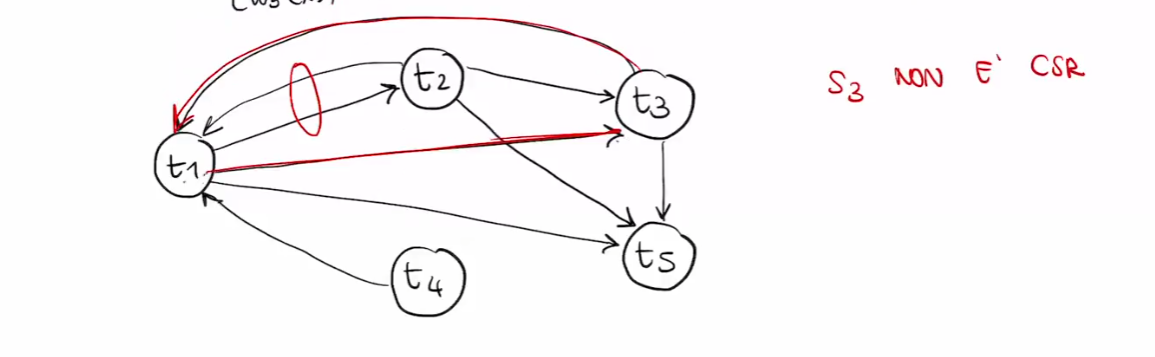
\includegraphics[width=0.7\linewidth]{image244}
	\label{fig:image244}
\end{figure}
Il grafo contiene cicli, ad esempio $t_1 \to t_2 \to t_1$ (dagli archi $t_1 \to t_2$ e $t_2 \to t_1$) e $t_2 \to t_3 \to t_1 \to t_2$. Il grafo è quindi ciclico, pertanto $S_3$ non è CSR. Poiché avevamo già dimostrato che $S_3$ non è VSR, concludiamo che $\mathbf{S_3}$ \textbf{non è né CSR né VSR}.
\paragraph{Esempio CSR: schedule $S_4$.}

Consideriamo lo schedule:
\[
S_4 : r_1(x),\ r_3(y),\ w_1(y),\ w_4(x),\ w_1(t),\ w_5(x),\ r_2(z),\ r_3(z),\ w_2(z),\ w_5(z),\ r_4(t),\ r_5(t)
\]

Costruiamo l'insieme dei conflitti:
\begin{align*}
	\text{CONFLITTI}(S_4) = \{
	&(r_1(x),\ w_4(x)),\ (r_1(x),\ w_5(x)), \\
	&(r_3(y),\ w_1(y)), \\
	&(w_4(x),\ w_5(x)), \\
	&(w_1(t),\ r_4(t)),\ (w_1(t),\ r_5(t)), \\
	&(r_2(z),\ w_5(z)), \\
	&(r_3(z),\ w_2(z)),\ (r_3(z),\ w_5(z)), \\
	&(w_2(z),\ w_5(z))
	\}
\end{align*}

Ricaviamo gli archi del grafo dei conflitti:
\begin{itemize}
	\item $(r_1(x),\ w_4(x))$, $(r_1(x),\ w_5(x))$ $\Rightarrow$ archi $t_1 \to t_4$, $t_1 \to t_5$;
	\item $(r_3(y),\ w_1(y))$ $\Rightarrow$ arco $t_3 \to t_1$;
	\item $(w_4(x),\ w_5(x))$ $\Rightarrow$ arco $t_4 \to t_5$;
	\item $(w_1(t),\ r_4(t))$, $(w_1(t),\ r_5(t))$ $\Rightarrow$ archi $t_1 \to t_4$, $t_1 \to t_5$;
	\item $(r_2(z),\ w_5(z))$ $\Rightarrow$ arco $t_2 \to t_5$;
	\item $(r_3(z),\ w_2(z))$, $(r_3(z),\ w_5(z))$ $\Rightarrow$ archi $t_3 \to t_2$, $t_3 \to t_5$;
	\item $(w_2(z),\ w_5(z))$ $\Rightarrow$ arco $t_2 \to t_5$.
\end{itemize}
\begin{figure}[H]
	\centering
	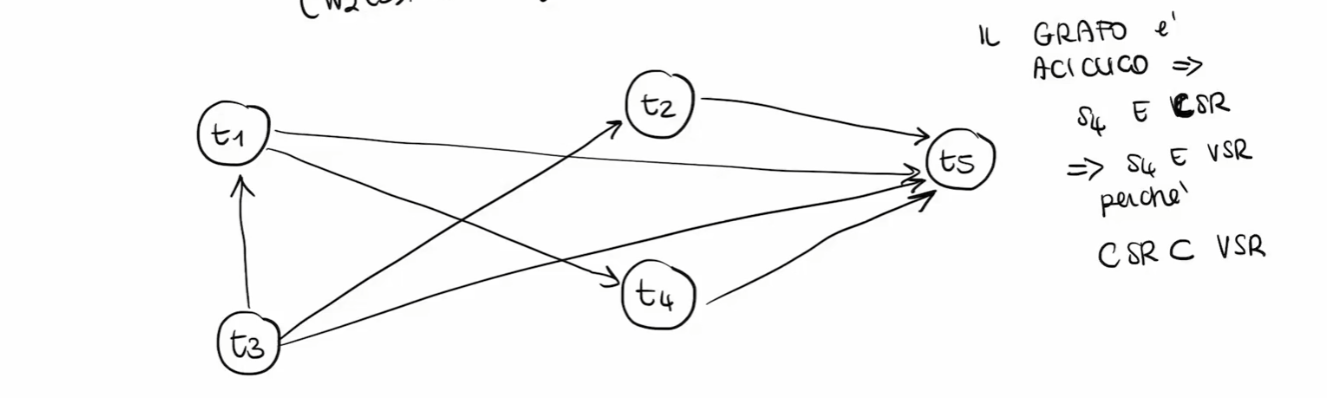
\includegraphics[width=0.7\linewidth]{image245}
	\caption{}
	\label{fig:image245}
\end{figure}
Il grafo dei conflitti ha quindi archi: $t_3 \to t_1 \to t_4 \to t_5$, $t_3 \to t_2 \to t_5$, $t_1 \to t_5$, $t_3 \to t_5$. Il grafo è \textbf{aciclico}, pertanto $S_4$ è CSR. Poiché $\text{CSR} \subseteq \text{VSR}$, concludiamo che $\mathbf{S_4}$ \textbf{è sia CSR che VSR}.
\paragraph{Ordinamenti topologici di $S_4$.}

Poiché il grafo dei conflitti di $S_4$ è aciclico, possiamo ricavare gli schedule seriali conflict-equivalenti tramite l'ordinamento topologico. Il nodo di partenza è $t_3$, l'unico senza archi entranti. I possibili ordinamenti topologici sono:

\begin{align*}
	S_{r1} &: t_3,\ t_1,\ t_5,\ t_2,\ t_4 \\
	S_{r2} &: t_3,\ t_1,\ t_5,\ t_4,\ t_2 \\
	S_{r3} &: t_3,\ t_2,\ t_1,\ t_4,\ t_5
\end{align*}

Tutti e tre gli schedule seriali sono conflict-equivalenti e view-equivalenti a $S_4$.
\subsection{Locking a due fasi stretto (2PL stretto)}

Il locking a due fasi stretto è il meccanismo principale per la gestione della concorrenza nei DBMS. I suoi vantaggi rispetto alla view-serializzabilità sono:
\begin{itemize}
	\item non richiede di conoscere in anticipo l'esito delle transazioni;
	\item fornisce un meccanismo base per la gestione dei lock;
	\item definisce una politica di concessione dei lock;
	\item garantisce la serializzabilità tramite una regola precisa.
\end{itemize}

\subsubsection{Meccanismo di base}

Per bloccare le risorse su cui si vuole operare si introducono le seguenti primitive di lock:
\begin{itemize}
	\item \textbf{R\_LOCK$_i(x)$}: la transazione $t_i$ richiede un lock condiviso in lettura sulla risorsa $x$;
	\item \textbf{W\_LOCK$_i(x)$}: la transazione $t_i$ richiede un lock esclusivo in scrittura sulla risorsa $x$;
	\item \textbf{UNLOCK$_i(x)$}: la transazione $t_i$ rilascia la risorsa $x$ da un precedente lock.
\end{itemize}

\paragraph{Regole d'uso delle primitive.}
\begin{itemize}
	\item Ogni operazione di \textbf{lettura} deve essere preceduta da una R\_LOCK e seguita da una UNLOCK. Sono ammessi più R\_LOCK contemporanei sulla stessa risorsa, poiché il lock in lettura è \textbf{condiviso}.
	\item Ogni operazione di \textbf{scrittura} deve essere preceduta da una W\_LOCK e seguita da una UNLOCK. Non sono ammessi più W\_LOCK contemporanei sulla stessa risorsa, poiché il lock in scrittura è \textbf{esclusivo}.
\end{itemize}

Una transazione che rispetta queste regole si dice \textbf{ben formata}.

\subsubsection{Politica di concessione dei lock}

Il gestore della concorrenza del DBMS mantiene per ogni risorsa $x$ le seguenti informazioni:
\begin{itemize}
	\item $\text{stato}(x) \in \{\text{libero},\ \text{r\_lock},\ \text{w\_lock}\}$: lo stato corrente della risorsa;
	\item $C(x) = \{t_1, \ldots, t_n\}$: l'insieme delle transazioni che detengono un R\_LOCK su $x$ (rilevante solo quando $\text{stato}(x) = \text{r\_lock}$).
\end{itemize}
\begin{figure}[H]
	\centering
	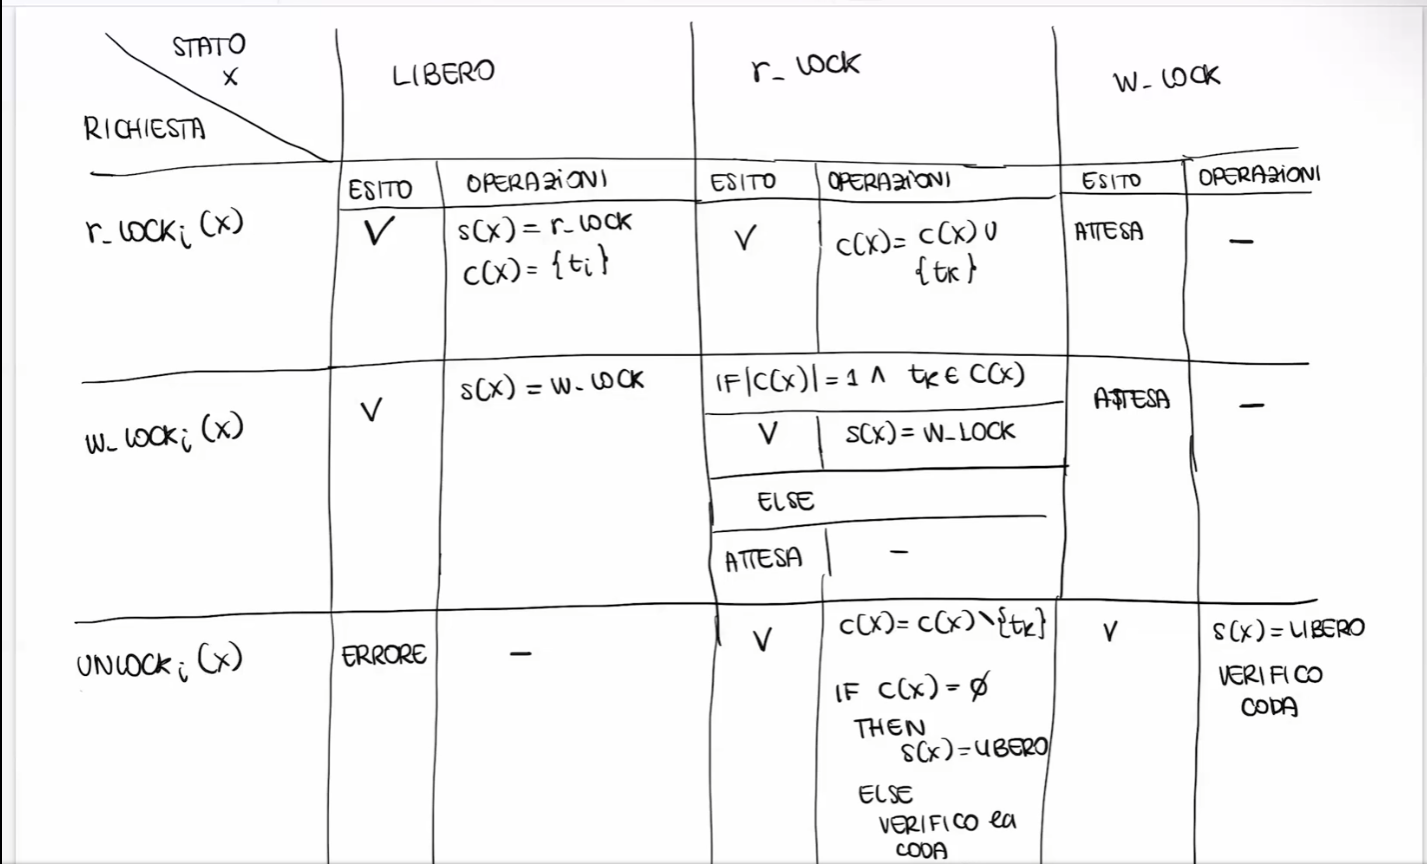
\includegraphics[width=1\linewidth]{image246}
	\caption{Tabella di concessione dei lock}
	\label{fig:image246}
\end{figure}
\subsection{Regola per la serializzabilità}

La regola da cui si ottiene la serializzabilità, e da cui deriva il nome \textit{2PL}, stabilisce che \textbf{una transazione, dopo aver rilasciato un lock, non può acquisirne altri}.

Il ciclo di vita di una transazione è suddiviso in due fasi distinte:

\begin{enumerate}
	\item \textbf{Fase di acquisizione (Growing Phase):} il numero di lock acquisiti cresce monotonicamente.
	\item \textbf{Fase di rilascio (Shrinking Phase):} il numero di lock decresce monotonicamente; non è più possibile acquisire nuovi lock.
\end{enumerate}

\begin{figure}[H]
	\centering
	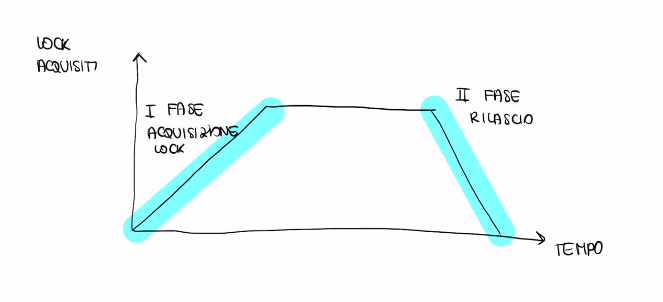
\includegraphics[width=1\linewidth]{image247}
	\caption{ciclo vita lock}
	\label{fig:image247}
\end{figure}

\paragraph{Esempio: perdita di aggiornamento con 2PL stretto.}

Consideriamo le transazioni:
\begin{align*}
	t_1 &: \text{R\_LOCK}_1(x),\ r_1(x),\ \text{W\_LOCK}_1(x),\ w_1(x),\ \text{UNLOCK}_1(x) \\
	t_2 &: \text{R\_LOCK}_2(x),\ r_2(x),\ \text{W\_LOCK}_2(x),\ w_2(x),\ \text{UNLOCK}_2(x)
\end{align*}

Lo schedule con perdita di aggiornamento era:
\[
S_{pa} : r_1(x),\ r_2(x),\ w_2(x),\ w_1(x)
\]

Con il 2PL stretto, introduciamo esplicitamente le operazioni di lock:
\[
S_{pa}^{2PL} : \text{R\_LOCK}_1(x),\ r_1(x),\ \text{R\_LOCK}_2(x),\ r_2(x),\ \text{W\_LOCK}_2(x)\ [\text{?}],\ \ldots
\]

Quando $t_2$ tenta di acquisire W\_LOCK$_2(x)$, lo stato della risorsa è:
\[
\text{stato}(x) = \texttt{r\_lock}, \quad C(x) = \{t_1,\ t_2\}
\]

Dalla tabella di concessione, W\_LOCK$_2(x)$ è concedibile solo se $C(x) = \{t_2\}$, ovvero se $t_1$ ha già rilasciato il proprio R\_LOCK$_1(x)$. Tuttavia:

\begin{itemize}
	\item Se $t_1$ rilascia R\_LOCK$_1(x)$, entra nella \textbf{fase discendente} del 2PL.
	\item Nella fase discendente, $t_1$ non può più acquisire nuovi lock.
	\item Ma $t_1$ deve ancora eseguire $w_1(x)$, che richiede W\_LOCK$_1(x)$: \textbf{impossibile}.
\end{itemize}

Il 2PL stretto impedisce quindi strutturalmente lo schedule $S_{pa}$: non esiste alcun modo di ordinare le operazioni di lock e unlock che rispetti contemporaneamente la regola del 2PL e consenta l'esecuzione di entrambe le scritture. La perdita di aggiornamento viene così \textbf{prevenuta}.
\subsubsection{2PL stretto}

Il \textbf{2PL stretto} aggiunge un vincolo ulteriore rispetto al 2PL base: una transazione può rilasciare i propri lock \textbf{esclusivamente dopo aver eseguito un commit o un rollback}. Il momento in cui inizia la fase discendente coincide quindi con il commit o l'abort della transazione.

Questo vincolo aggiuntivo permette di \textbf{eliminare l'ipotesi di commit-proiezione}: il 2PL stretto garantisce la serializzabilità anche in presenza di transazioni che terminano con un abort, senza dover assumere a priori l'esito delle transazioni.

\subsubsection{Relazione tra 2PL stretto, CSR e VSR}

I tre insiemi di schedule sono in relazione di inclusione stretta:
\[
\text{2PL stretto} \subsetneq \text{CSR} \subsetneq \text{VSR}
\]

\begin{itemize}
	\item Ogni schedule prodotto dal 2PL stretto è conflict-serializzabile, ma non tutti gli schedule CSR sono producibili dal 2PL stretto.
	\item Ogni schedule CSR è view-serializzabile, ma non tutti gli schedule VSR sono conflict-serializzabili.
\end{itemize}

Il 2PL stretto è quindi la condizione più restrittiva: sacrifica parte della concorrenza ammessa da CSR e VSR, ma in cambio offre un meccanismo \textbf{pratico, efficiente e privo di ipotesi sull'esito delle transazioni}.
\subsection{Blocco critico (Deadlock)}

Il \textbf{blocco critico} (o \textit{deadlock}) si verifica durante l'esecuzione concorrente di due o più transazioni quando si crea una situazione di attesa circolare:
\begin{itemize}
	\item $t_1$ detiene una risorsa di cui $t_2$ ha bisogno, ed è in attesa di una risorsa detenuta da $t_2$;
	\item $t_2$ detiene una risorsa di cui $t_1$ ha bisogno, ed è in attesa di una risorsa detenuta da $t_1$.
\end{itemize}
Nessuna delle due transazioni può proseguire.

\paragraph{Frequenza del deadlock.}
Assumendo una granularità del lock a livello di tupla e indicando con $N$ il numero medio di tuple per tabella, la probabilità di deadlock di lunghezza due è:
\[
P(\text{deadlock}) = \frac{1}{N^2}
\]
All'aumentare del numero di tuple la probabilità decresce: con granularità fine il deadlock è un evento raro.

\paragraph{Tecniche di gestione.}

\begin{enumerate}
	\item \textbf{Timeout}: una transazione in attesa di una risorsa viene abortita allo scadere di un intervallo di tempo prefissato. È la tecnica più semplice da implementare, ma può abortire transazioni che non sono effettivamente in deadlock.
	
	\item \textbf{Prevenzione}: ogni transazione acquisisce \textbf{tutte} le risorse di cui necessita in lettura e scrittura in un'unica soluzione, secondo una politica del tutto-o-niente. Elimina il deadlock alla radice, ma è molto costosa in termini di concorrenza, poiché le risorse vengono bloccate anche quando non sono ancora necessarie.
	
	\item \textbf{Rilevamento}: è la tecnica adottata nella maggior parte dei sistemi reali. Periodicamente il sistema analizza la tabella dei lock alla ricerca di cicli di attesa; se viene rilevato un deadlock, una delle transazioni coinvolte viene abortita per spezzare il ciclo. Lo svantaggio è il rischio di \textbf{starvation}: la stessa transazione potrebbe essere ripetutamente scelta come vittima e non riuscire mai a completare.
\end{enumerate}
\subsection{Livelli di isolamento}

Esiste un compromesso fondamentale tra il grado di isolamento dalle anomalie e le prestazioni del sistema (misurate in TPS): maggiore è il controllo della concorrenza, minore è il parallelismo ammesso e quindi le prestazioni. I DBMS consentono di rinunciare, in tutto o in parte, al controllo della concorrenza, specificando quali anomalie si è disposti a tollerare tramite i \textbf{livelli di isolamento}.

\begin{figure}[H]
	\centering
	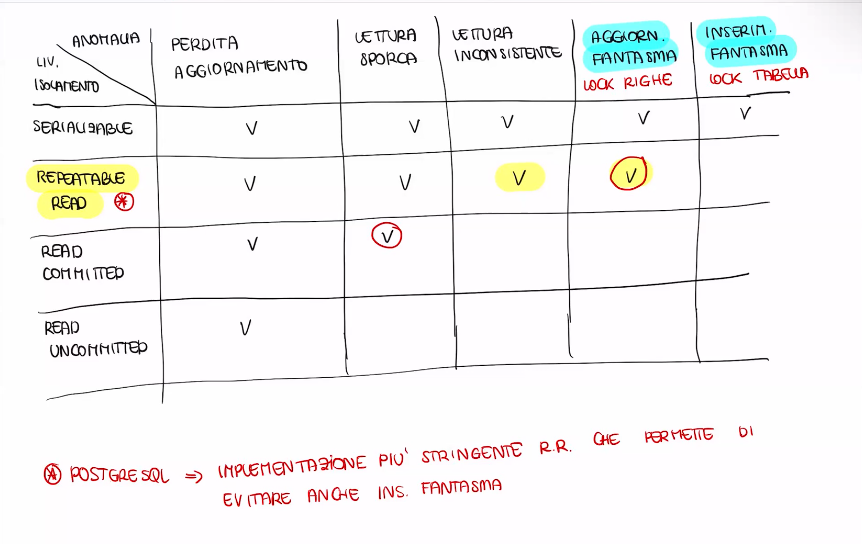
\includegraphics[width=1\linewidth]{image248}
	\caption{Anomalie evitate (\checkmark) per ciascun livello di isolamento}
	\label{fig:image248}
\end{figure}

\noindent$^*$ \textit{PostgreSQL} adotta un'implementazione più stringente del livello Repeatable Read, che permette di evitare anche l'inserimento fantasma.

Al livello più alto (\textbf{Serializable}) tutte le anomalie sono prevenute; scendendo di livello si tollerano anomalie via via più gravi, guadagnando in concorrenza e prestazioni.
\subsubsection{Implementazione dei livelli di isolamento}

Tutti i livelli di isolamento richiedono il \textbf{2PL stretto per le scritture}: i lock in scrittura vengono sempre rilasciati solo dopo il commit o il rollback. I livelli si differenziano invece nella gestione dei lock in lettura.

\begin{itemize}
	\item \textbf{Serializable}: applica il 2PL stretto anche per le letture e acquisisce lock a livello di \textbf{tabella}, prevenendo così l'anomalia di inserimento fantasma.
	
	\item \textbf{Repeatable Read}: applica il 2PL stretto anche per le letture, ma acquisisce lock a livello di \textbf{tupla} anziché di tabella. Previene la lettura inconsistente e l'aggiornamento fantasma, ma ammette l'anomalia di inserimento fantasma.
	
	\item \textbf{Read Committed}: acquisisce lock condivisi in lettura, ma \textbf{non} segue la regola del 2PL stretto per essi: i lock in lettura vengono rilasciati non appena l'operazione di lettura è completata, senza attendere il commit. Previene la lettura sporca, ma ammette la lettura inconsistente.
	
	\item \textbf{Read Uncommitted}: non acquisisce alcun lock in lettura. È il livello con la massima concorrenza, ma ammette tutte le anomalie di lettura, compresa la lettura sporca.
\end{itemize}